\documentclass[11pt, letterpaper]{article}
\input{/home/hyperion/.config/LatexHub/preambles/base.tex}
\input{/home/hyperion/.config/LatexHub/preambles/diagrams.tex}
\input{/home/hyperion/.config/LatexHub/preambles/tikz.tex}
\input{/home/hyperion/.config/LatexHub/preambles/macros-cat-theory.tex}
\input{/home/hyperion/.config/LatexHub/preambles/macros-algebra.tex}
\input{/home/hyperion/.config/LatexHub/preambles/basic-theorems-section.tex}
\input{/home/hyperion/.config/LatexHub/preambles/refs-basic.tex}
\input{/home/hyperion/.config/LatexHub/preambles/physics.tex}
\input{/home/hyperion/.config/LatexHub/preambles/code.tex}
\usepackage{titlepageBU}
\title{Midterm 2}
\begin{document}
\makeproblem
\part{Quickies}
\section{Plotting momentum space wavefunction: harmonic oscillator}
The first excited momentum space wavefunction $\phi _1(p)=\braket{p}{1}$ is
\[
	\phi _1(p)=\left( \frac{1}{\pi m\hbar \omega }  \right) ^{1/4}  \frac{p\sqrt{2}}{\sqrt{m\hbar\omega } } \exp \left( -\frac{p^2}{2m\hbar\omega }  \right) 
.\]
Let $p_0=\sqrt{m\omega \hbar} $ to simplify notation, such that
\[
	\phi _1(p) = \left( \frac{1}{\pi p_0^2 }  \right) ^{1/4} \frac{p \sqrt{2} }{p_0} \exp \left( -\frac{p^2}{2p_0^2}  \right) 
.\]
Then
\[
	\left| \phi _1(p) \right| ^2 = \frac{1}{\sqrt{\pi p_0^2} } \frac{2p^2}{p_0^2} \exp \left( -\frac{p^2}{p_0^2}  \right) =\frac{2p^2}{p_0^3 \sqrt{\pi } } \exp \left( -\frac{p^2}{p_0^2}  \right) 
.\]
We set $m=\omega =\hbar=1$ in our plot. 
\begin{lstlisting}[language=Python]
#!/bin/python3

import numpy as np
import matplotlib.pyplot as plt

# natural units
m = 1.0
omega = 1.0
hbar = 1.0

p0 = np.sqrt(m * hbar * omega)

p = np.linspace(-5 * p0, 5 * p0, 1000)

prob_density = 2 * (p**2) * np.exp(-(p**2) / (p0**2)) / ((p0**3) * np.sqrt(np.pi))

# plotting
plt.figure(figsize=(8, 6))
plt.plot(p, prob_density, color='black', linewidth=1.5)

plt.xlabel(r'$p = \hbar k$', fontsize=14)
plt.ylabel(r'$|\langle p | 1 \rangle|^2$', fontsize=14)
plt.title(r'Momentum Space Probability Density: First Excited State ($n=1$)', fontsize=14)

plt.grid(True, linestyle='--', alpha=0.7)
plt.tight_layout()
plt.savefig('asnjddsnfjk.png')
\end{lstlisting}
\begin{figure}[ht]
	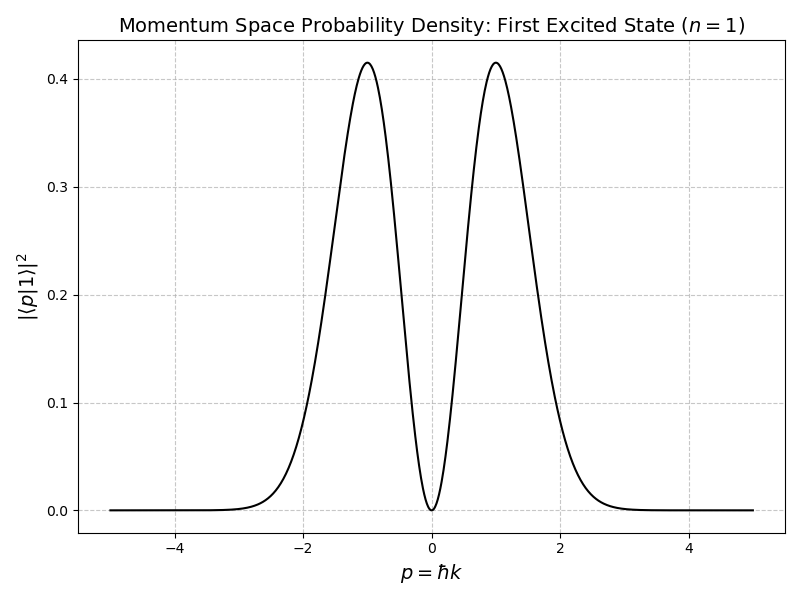
\includegraphics[scale=0.8]{./asnjddsnfjk.png}
	\centering
	\caption{Momentum space probability density for first excited state $\ket{n}=\ket{1}$}
	\centering
\end{figure}


\section{Interaction potential}
We use Hadamard's operator lemmma
\[
	e^{A} Be^{-A}= B + [A,B] + \frac{1}{2} [A,[A,B]] + \cdots
\]
with $A=iH_0t/\hbar$ and $B=V $. We then use the identities
\[
	[AB,C]=A[B,C]+[A,C]B,
\]
\[
	[A,BC]=[A,B]C+B[A,C]
\]
to compute
\[
	[\hat{x} ^2,\hat{p} ^2]=\hat{x} [\hat{x} ,\hat{p} ^2] + [\hat{x} ,\hat{p} ^2]\hat{x} =\hat{x} \left( [\hat{x} ,\hat{p} ]\hat{p} +\hat{p} [\hat{x} ,\hat{p} ] \right) +\left( [\hat{x} ,\hat{p} ]\hat{p} +\hat{p} [\hat{x} ,\hat{p} ] \right)\hat{x} =2i\hbar\hat{x} \hat{p}+2i\hbar \hat{p} \hat{x} 
.\]
We then have
\[
	[iH_0t/\hbar,V]=\left[ \frac{i t\hat{p} ^2}{2m\hbar} ,\frac{m\omega _0^2 \hat{x} ^2}{2}  \right] =\frac{it\omega _0^2}{4\hbar} [\hat{p} ^2,\hat{x} ^2]= -\frac{it\omega _0^2}{4\hbar} [\hat{x} ^2,\hat{p} ^2]=\frac{t\omega _0^2}{2} \left\{ \hat{x} ,\hat{p}  \right\} 
\]
for $\left\{ -,- \right\} $ the anticommutator. We then compute
\[
	[iH_0t/\hbar,[iH_0t/\hbar,V]]= \frac{t\omega _0^2}{2} \left[\frac{it\hat{p} ^2}{2m\hbar}, \left\{ \hat{x},\hat{p}  \right\} \right]=\frac{it^2\omega _0^2}{4m\hbar} \left[ \hat{p} ^2,\left\{ \hat{x} ,\hat{p}  \right\}  \right] 
.\]
We compute the commutator independently in order to not keep rewriting the coefficient.
\[
	[\hat{p} ^2,\hat{p} \hat{x} +\hat{x} \hat{p} ]=[\hat{p} ^2,\hat{p} \hat{x} ]+[\hat{p} ^2,\hat{x} \hat{p} ]=[\hat{p} ^2,\hat{p} ]\hat{x} +\hat{p} [\hat{p} ^2,\hat{x} ]+[\hat{p} ^2,\hat{x} ]\hat{p} +\hat{x} [\hat{p} ^2,\hat{p} ]=\hat{p} [\hat{p} ^2,\hat{x} ]+[\hat{p} ^2,\hat{x} ]\hat{p} 
.\]
We can compute $[\hat{p} ^2,\hat{x} ]$:
\[
	[\hat{p} ^2,\hat{x} ]=\hat{p} [\hat{p} ,\hat{x} ]+[\hat{p} ,\hat{x} ]\hat{p} =-2i\hbar \hat{p} 
.\]
We thus obtain
\[
	[\hat{p} ^2, \left\{ \hat{p} ,\hat{x}  \right\} ]=\hat{p} (-2i\hbar \hat{p} ) + (-2i\hbar \hat{p} )\hat{p} =-4i\hbar \hat{p} ^2
.\]
The full term is thus
\[
	\frac{1}{2} \frac{it^2\omega _0^2}{4m\hbar} (-4i\hbar )\hat{p} ^2 = \frac{t^2\omega _0^2}{2m} \hat{p} ^2
.\]

Since $\hat{p} $ commutes with itself, all higher order terms vanish, so we obtain
\[
	V_I = \frac{m\omega _0^2}{2} \hat{x} ^2 + \frac{t\omega _0^2}{2} \left\{ \hat{x} ,\hat{p}  \right\} + \frac{t^2 \omega _0^2}{2m} \hat{p} ^2
.\]


\section{Josephson-junction}

We are given $V=v_0 \cos \omega t$. Applying this to the time-evolution of $\phi _2-\phi _1$ gives
\[
	\frac{\partial (\phi _2-\phi _1)}{\partial t} =\frac{2e}{\hbar} v_0 \cos \omega t
.\]
Integrating and assuming the junction has no initial phase difference yields
\[
	\phi _2-\phi _1=\frac{2e}{\hbar}\frac{\hbar\omega }{2e}  \int \cos \omega t \,\mathrm{d} t=\sin \omega t
.\]
We then obtain
\[
	I(t)=I_c \sin (\sin (\omega t))
.\]
We plot the current $I(t)$ as a function of $\tau =\omega t$ over two periods. We take $I_c=1$ for simplicity.
\begin{lstlisting}[language=Python]
#!/bin/python3

import numpy as np
import matplotlib.pyplot as plt

# take tau to be omega*t
tau = np.linspace(0, 4 * np.pi, 1000)

# take I_c=1
current = np.sin(np.sin(tau))

# 4. Plotting
fig, ax = plt.subplots(figsize=(8, 6))
    
ax.plot(tau, current, 'k-', linewidth=1.5, label=r'$I(t) = I_c \sin(\sin(\omega t))$')
    
ax.set_xlabel(r'$\omega t$ (rad)', fontsize=12)
ax.set_ylabel(r'Current $I(t)$', fontsize=12)
    
# just make it look a lil nicer
ax.axhline(0, color='gray', linestyle='--', linewidth=0.8, alpha=0.7)
ax.grid(True, which='both', linestyle=':', alpha=0.6)
ax.set_xlim(0, 4 * np.pi)
ax.set_ylim(-1.1, 1.1)
ax.legend(loc='upper right', frameon=True)

plt.savefig('josephson_current.png', dpi=300)
plt.show()
\end{lstlisting}
\begin{figure}[ht]
	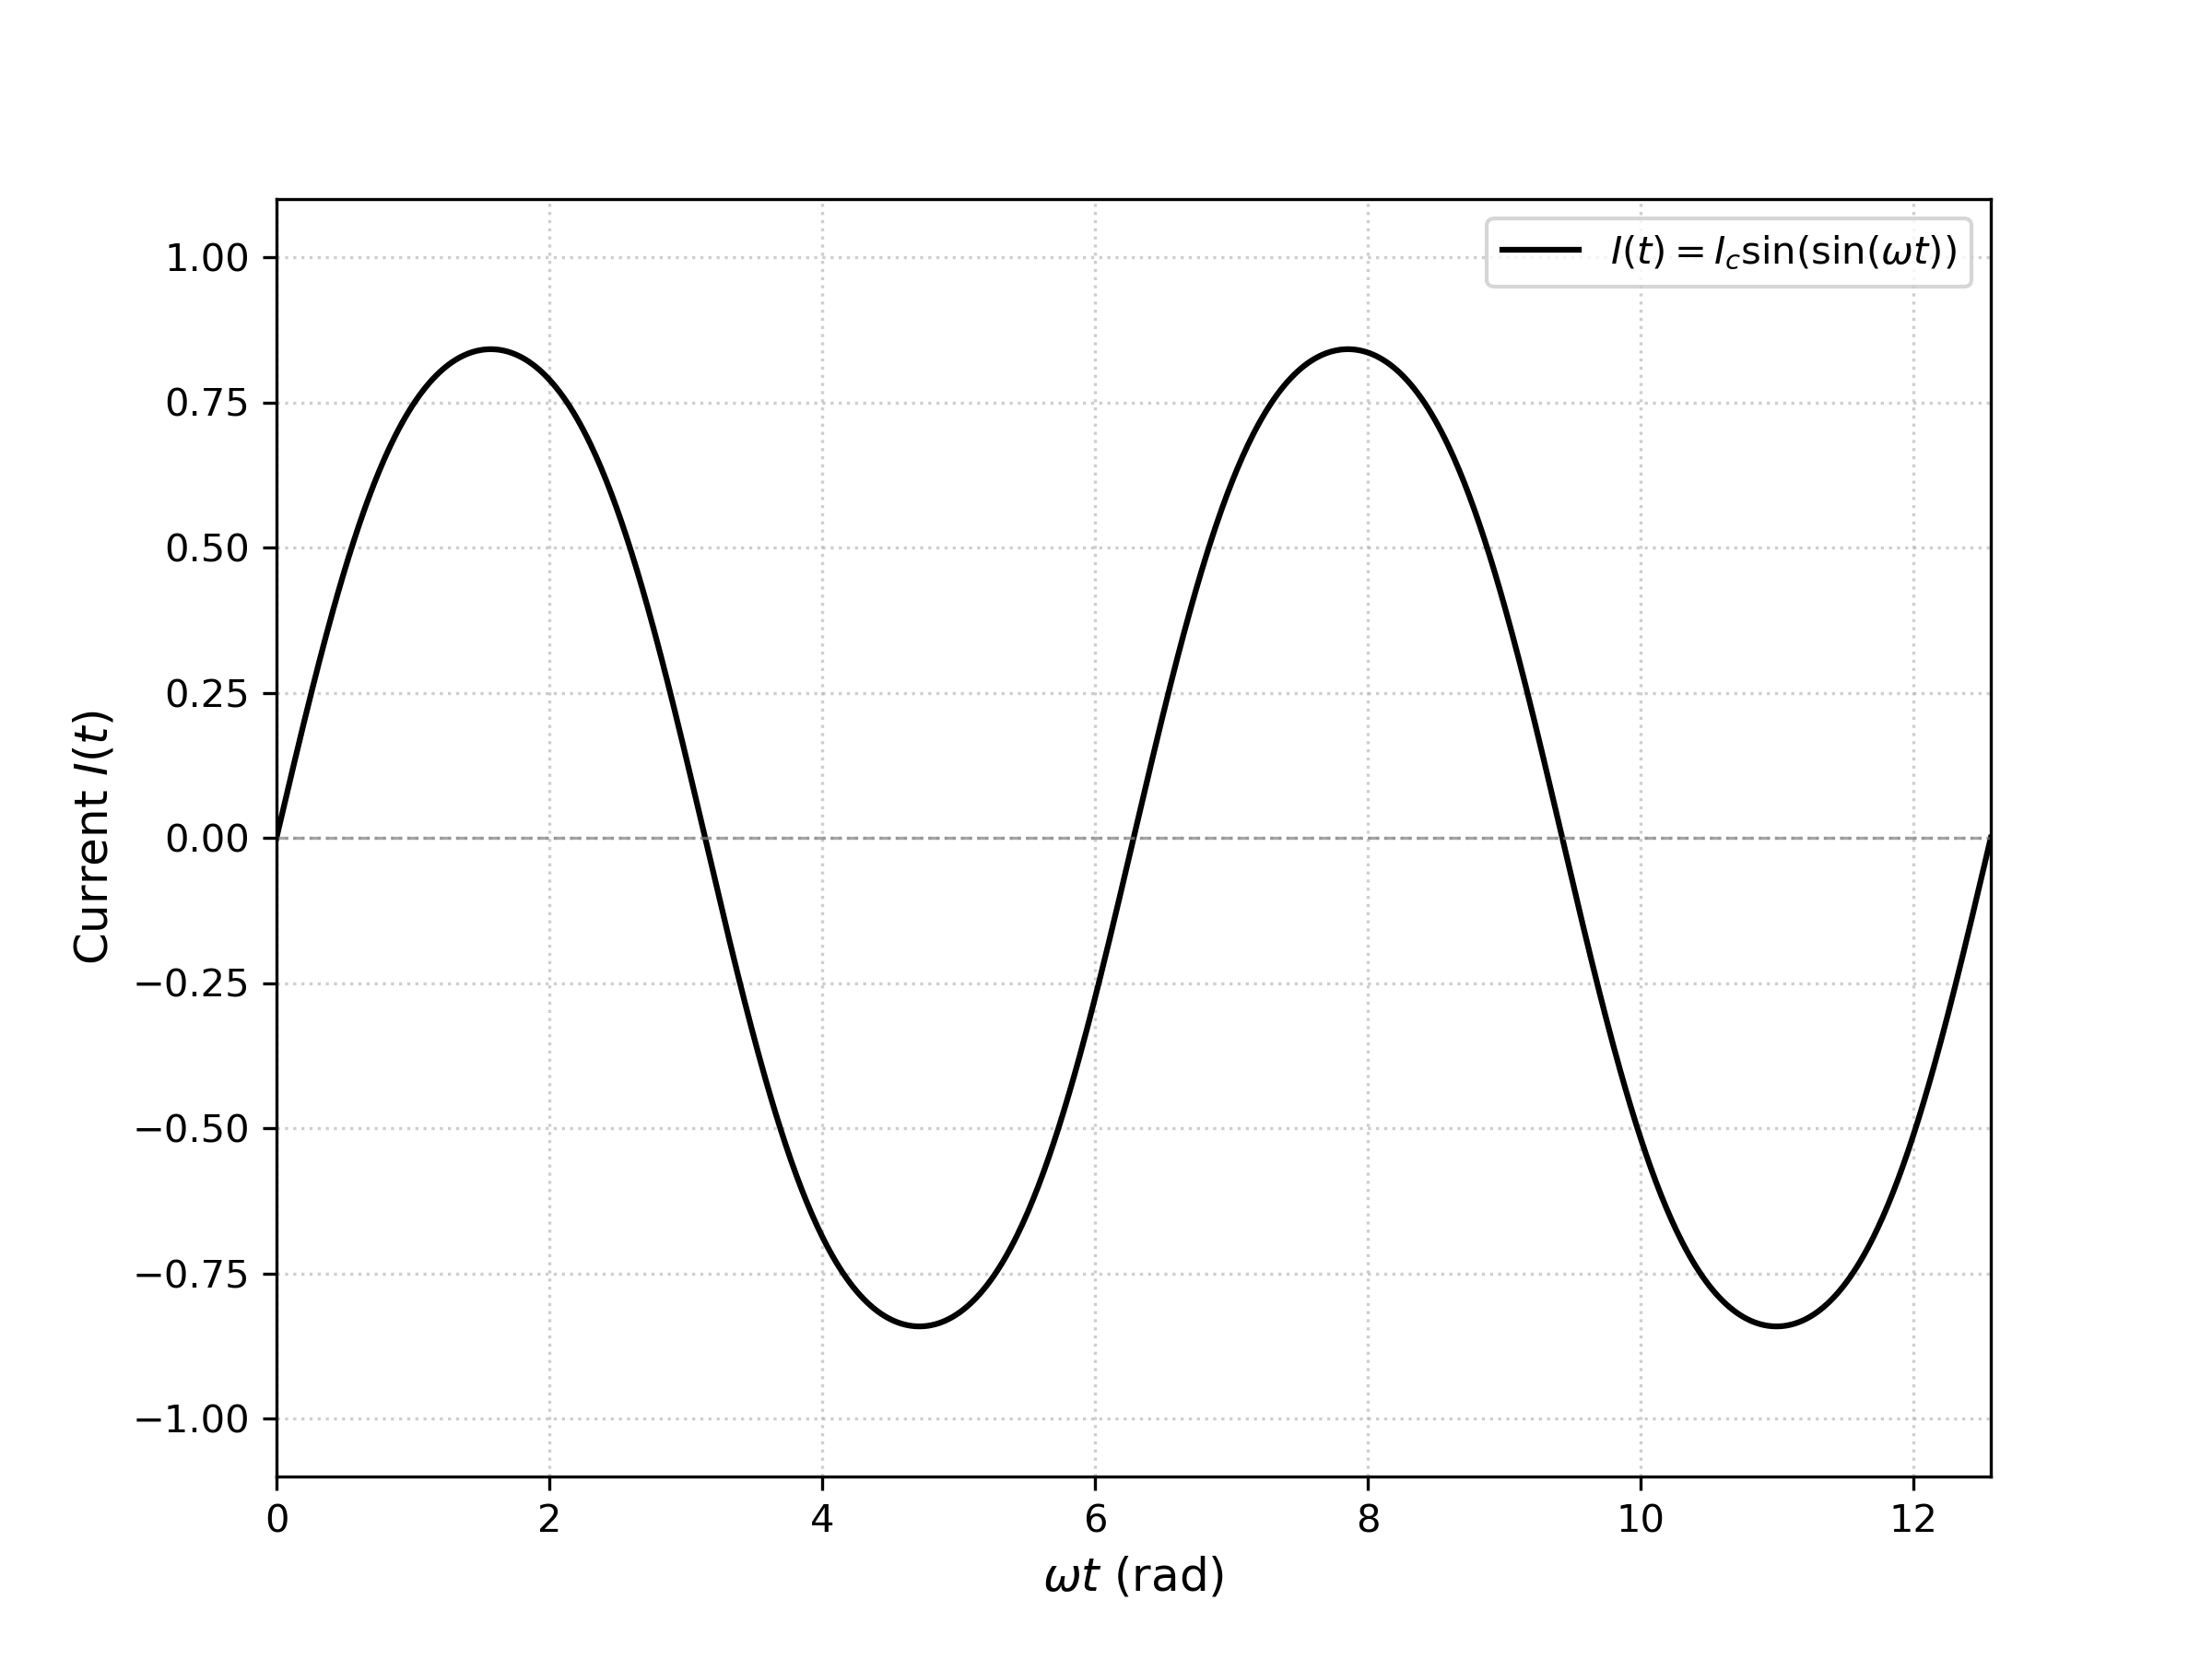
\includegraphics[scale=0.8]{./josephson_current.png}
	\centering
	\caption{The current $I$ of the Josephson junction plotted along 2 periods against $\omega t$.}
	\centering
\end{figure}


The function $\sin (\sin (\omega t))$ is an odd periodic function, as seen in the figure, and its average value over one period is also seen to be 0. Thus there is no DC current.

\section{Displacement operator}
(i) Alfie's translation operators send $\hat{D} (-\alpha )\ket{\alpha }=\ket{\alpha -\alpha }=\ket{0}$ and $\hat{D} (-\beta )\ket{0}=\ket{-\beta }\neq \ket{\beta }$. Therefore Alfie's setup is wrong.

(ii) Betty deserves full credit. Since $\hat{D} $ is unitary, its inverse is given by $\hat{D} ^\dagger$. Since $\hat{D} (\alpha )\ket{0}=\ket{\alpha }$, its inverse acts by $\hat{D} ^\dagger\ket{\alpha }=\ket{0}$. We then have $\hat{D} (\beta )\ket{0}=\ket{\beta }$. Therefore, Betty's transformations indeed map $\ket{\alpha }\mapsto \ket{\beta }$.

(iii) Gammy's setup is also wrong.
\[
	\hat{D} (\alpha )\hat{D} (\beta )\ket{\alpha }=\hat{D} (\alpha )\ket{\beta +\alpha }=\ket{2\alpha +\beta }\neq \ket{\beta }
.\]

(iv) Delter's setup is correct. Noting again that $\hat{D} ^\dagger(z ) = \hat{D} ^{-1} (z)=\hat{D} (-z)$ for any $z$,
\[
	\hat{D} ^\dagger(-\beta )\hat{D} ^\dagger(\alpha )\ket{\alpha }=\hat{D} (\beta )\hat{D} (-\alpha )\ket{\alpha }=\hat{D} (\beta )\ket{0}=\ket{\beta }
.\]

(v) Epsom's setup is wrong.
\[
	\hat{D} ^\dagger(\alpha )\hat{D} ^\dagger(\beta )\ket{\alpha }=\hat{D} (-\alpha )\hat{D} (-\beta )\ket{\alpha }=\hat{D} (-\alpha )\ket{\alpha -\beta }=\ket{-\beta }\neq \ket{\beta }
.\]
\section{Quantum LC circuit}
(i) In an LC circuit the angular frequency is $\omega =\frac{1}{\sqrt{LC} } $. This yields $C=\frac{1}{\omega ^2L} $. We have $\omega =2\pi f = 2\pi (5\cdot 10^9)=10\pi \cdot 10^9$ rad$/$s. Then
\[
	C=\frac{1}{\left( 10^{-8} \mathrm{H}  \right) \left( 10\pi \cdot 10^9 \mathrm{rad} /\mathrm{s}  \right)^2 } =\frac{1}{10^{12} \pi ^2} \mathrm{F} \approx 1\cdot 10^{-13} \mathrm{F} 
.\]

(ii) No.

(iii) No, due to the uncertainty principle. There is a conjugation relation $[\hat{\Phi },\hat{Q} ]=i\hbar$, and thus an uncertainty principle
\[
	\Delta \Phi \Delta Q \geq \frac{\hbar}{2} 
\]
is satisfied. To detect a cooper pair, the state would need to be in a Fock state of charge with small $\Delta Q$. To detect a flux quanta, the state would need to be in a Fock state of flux with small $\Delta \Phi $. The uncertainty principle forbids both quantities being small.
\part{Longer problems}
\section{Simple harmonic oscillator with perturbation in momentum}

(a) Because $\hat{H} $ is the \emph{energy} operator, $\lambda \hat{p} $ must have units of energy, meaning $\lambda $ must have units of velocity. For the perturbation to be \emph{weak}, we would want the induced energy shift to be significantly smaller than the energy gap between states. In the 1D harmonic oscillator with a nonperturbed Hamiltonian, the energy difference is $\Delta E=\hbar \omega _0$, so we want the perturbation to induce a much smaller energy change than this. Recall this is approximately $\lambda \sqrt{m\hbar\omega _0} $, so we have
\[
	\lambda \ll \frac{\hbar \omega _0}{\sqrt{m\hbar \omega _0} } =\sqrt{\frac{\hbar\omega _0}{m}}
.\]


(b) Start by rewriting the momentum-dependent terms of the Hamiltonian as
\[
	\frac{\hat{p} ^2}{2m} +\lambda \hat{p} =\frac{1}{2m} \left( \hat{p} ^2 + 2m\lambda \hat{p}  \right) 
.\]
We can complete the square:
\[
	=\frac{1}{2m} \left( \hat{p} ^2 + 2m\lambda \hat{p} +m^2\lambda ^2-m^2\lambda ^2 \right) =\frac{1}{2m} \left( \hat{p} +m\lambda  \right) ^2 - \frac{m\lambda^2 }{2} 
.\]
Substituting this back into the Hamiltonian, we have
\[
	\hat{H} =\frac{1}{2m} \left( \hat{p} + m\lambda  \right) ^2-\frac{m\lambda^2 }{2} +\frac{1}{2} m\omega _0^2 \hat{x} ^2
.\]
We define
\[
	\hat{X} \coloneqq \omega _0 \sqrt{m} \hat{x} 
\]
\[
	\hat{P} \coloneqq \frac{\hat{p} +m\lambda }{\sqrt{m} } 
\]
\[
	\text{constant} \coloneqq -\frac{m\lambda^2 }{2} 
.\]
The Hamiltonian then takes the form
\[
	\hat{H} =\frac{1}{2} \hat{P} ^2 + \frac{1}{2} \hat{X} ^2 + \text{constant} 
.\]

(c)
\begin{align*}
	[\hat{X} ,\hat{P} ]&=\left[ \omega _0 \sqrt{m} \hat{x} ,\frac{\hat{p} }{\sqrt{m}  } +\frac{m\lambda }{\sqrt{m} } \right] \\
			   &=\left[ \omega _0 \sqrt{m} \hat{x}, \frac{\hat{p} }{\sqrt{m} }   \right] + \left[ \omega _0 \sqrt{m} \hat{x} , \frac{m\lambda }{\sqrt{m} }  \right] \\
			   &=\left[ \omega _0 \sqrt{m} \hat{x} ,\frac{\hat{p} }{\sqrt{m} }  \right] \\
			   &=\omega _0 \left[ \hat{x} ,\hat{p}  \right] \\
			   &=i\hbar \omega _0
.\end{align*}

(d) Because the operators $\hat{X} ,\hat{P} $ have the commutation relation given in part (c), they must describe a harmonic oscillator with the same frequency $\omega _0$ as the unperturbed system. The energy eigenvalues are therefore the exact same as the standard oscillator eigenvalues
\[
	E_n=\hbar \omega _0\left( n+\frac{1}{2}  \right) 
.\]
The total energy of the perturbed system is thus just shifted by the constant term
\[
	E_n = \hbar\omega _0\left( n+\frac{1}{2}  \right) -\frac{m\lambda ^2}{2} 
.\]
The correction in any state induced by this perturbation is thus
\[
	\Delta E_n = -\frac{m\lambda ^2}{2} 
.\]
This includes the $n=1$ case.

\section{Landau problem, symmetric gauge}

(a) 
\[
	\mathbf{B} =\nabla \times \mathbf{A} =\left( \partial _y0 - \partial _z \frac{1}{2} B_0x \right) \mathbf{\hat{x} } -\left( \partial _x0+\partial _z\frac{1}{2} B_0y \right) \mathbf{\hat{y} } + \left( \partial _x\frac{1}{2} B_0x + \partial _y\frac{1}{2} B_0y \right) \mathbf{\hat{z} } =B_0\mathbf{\hat{z} } 
\]

(b) The Hamiltonian in the $xy$-plane will be given by
\begin{align*}
	\hat{H} &=\frac{1}{2m} \left( \hat{\mathbf{p} } -q \mathbf{A}  \right) ^2\\
		&=\frac{1}{2m} \left(\left( \hat{p} _x+\frac{qB_0y}{2} \right) ^2+  \left( \hat{p} _y - \frac{qB_0x}{2}  \right) ^2\right)\\
		&=\frac{1}{2m} \left( \hat{p}_x^2 +\frac{q^2B_0^2y^2}{4} +qB_0y \hat{p}_x\right) +\left( \hat{p} _y^2 + \frac{q^2B_0^2x^2}{4} -qB_0x \hat{p}_y \right) \\
		&=\frac{\hat{p} _x^2 + \hat{p} _y^2}{2m} +\frac{q^2B_0^2}{8m} \left( x^2+y^2 \right) +\frac{qB_0}{2m} \left( y \hat{p} _x - x \hat{p} _y \right) 
.\end{align*}
Note the angular momentum operator $\hat{L} _z = x \hat{p} _y -y \hat{p} _x$, and define $\omega \coloneqq \frac{qB_0}{2m} $. The Hamiltonian then reads as
\[
	\hat{H} =\frac{\hat{\mathbf{p} } ^2}{2m} +\frac{1}{2} m\omega ^2\left( x^2+y^2 \right) -\omega \hat{L} _z
.\]
The first two terms resemble that of a 2D oscillator with frequency $\omega $, but there is an extra $\omega \hat{L} _z$ term at the end.

(c) The Hamiltonian becomes
\[
	\hat{H} =\frac{\hat{\mathbf{p}^2 } }{2m} +\frac{1}{2} m\omega ^2 r^2 - \omega \hat{L} _z
.\]
Recall the Laplacian in polar coordinates in 2D is
\[
	\nabla ^2=\frac{\partial ^2}{\partial r^2} +\frac{1}{r} \frac{\partial }{\partial r} +\frac{1}{r^2} \frac{\partial ^2}{\partial \phi ^2} 
.\]
Additionally,
\[
	\hat{L} _z =-i\hbar \frac{\partial }{\partial \phi } 
.\]
The time-dependent Schr\"odinger equation is thus
\[
	i\hbar \frac{\partial }{\partial t} \Psi (x,y,t) = \left(-\frac{\hbar^2}{2m} \left( \frac{\partial ^2}{\partial r^2} +\frac{1}{r} \frac{\partial }{\partial r} +\frac{1}{r^2} \frac{\partial ^2}{\partial \phi ^2}  \right) +\frac{1}{2} m\omega r^2 + i\hbar \omega \frac{\partial }{\partial \phi } \right)\Psi (x,y,t)
.\]
The time-independent Schr\"odinger equation is
\[
	\left(-\frac{\hbar^2}{2m} \left( \frac{\partial ^2}{\partial r^2} +\frac{1}{r} \frac{\partial }{\partial r} +\frac{1}{r^2} \frac{\partial ^2}{\partial \phi ^2}  \right) +\frac{1}{2} m\omega r^2 + i\hbar \omega \frac{\partial }{\partial \phi } \right)\psi (x,y)=E\psi (x,y)
.\]

(d) There is a degeneracy. The usual oscillator has energy eigenvalues $\hbar \omega (2n+|m|+1)$, but since $\hat{L} _z$ has an eigenvalue of $m\hbar$, the $-\omega \hat{L} _z$ term shifts the eigenvalues to
\[
	\hbar \omega (2n+|m|+1) - \omega m\hbar
.\]
Taking $n=0$ and $m\geq 0$ yields $E_0 = \hbar \omega $. We let $m$ range over all integers, and in particular positive integers, and we have shown for each positive integer there is a ground state with the same energy eigenvalue $\hbar \omega $.

\end{document}
